%\documentclass[twocolumn,floatfix,amsmath,amssymb,prb,showpacs,superscriptaddress,hyperref]{revtex4-2}
\documentclass{iopart}
\usepackage{iopams}
\expandafter\let\csname equation*\endcsname\relax
\expandafter\let\csname endequation*\endcsname\relax
\usepackage{amsmath}
\usepackage{amssymb}
\usepackage{caption}
\usepackage{amscd}
\usepackage{dsfont}
\usepackage{url}
\usepackage{graphicx}
%\graphicspath{{figs/}}
\usepackage{cite}
%\usepackage{graphicx}
\graphicspath{{./fig_paper/}}
\usepackage{hyperref}
\usepackage{color}
\usepackage{bbold}
\usepackage{tikz}\label{key}
\usepackage{dcolumn}
\usepackage{wasysym}
\usepackage{braket}
\usepackage{bm,listings}
%\usepackage{dsfont}
\usepackage[normalem]{ulem}
%\newcommand{\rmi}{{\rm i}}
%\newcommand{\rme}{{\rm e}}
%\newcommand{\rmd}{{\rm d}}
\usepackage{printlen}
\newcommand{\Dfancy}{\mathcal{D}}
\newcommand{\Afancy}{\hat{\mathcal{A}}}
\newcommand{\Sfancy}{\mathcal{S}}

\begin{document}
	
	\title{Multifractality and Chaos in a  PT-Symmetric Kicked Rotor}
	\date{\today}
	\author{Joseph Hall and Eva-Maria Graefe}
	\address{Department of Mathematics, Imperial College London, London, SW7 2AZ, United Kingdom}
	
	\begin{abstract}
	Quantum mechanics is a lie we tell each other to get payed.
	\end{abstract}
	\maketitle
	\bibliographystyle{iopart-num}

	\section{Introduction}

	\subsection{PT Hamiltonians}
	PT-symmetric Hamiltonians have been of great interest in recent years. Initially, this interest was due to their prized status as non-hermitian operators that, under certain conditions, could produce purely real spectrums. In these cases, despite the reality of the spectrum, the non-normality of the operator set them apart from their more familiar Hermitian counterparts. The eigenstates of the Hamiltonian are non-orthogonal leading to unique dynamical effects such as power oscillations. However, not all parametrisations of PT-symmetric Hamiltonians lead to purely real spectrums. In general, the spectrum is mixed and consist of both real and complex conjugate eigenvalues. Quantum mechanically the regime of mixed spectrum is of particular interest as the complex conjugate eigenvalues may be interpreted as gain and loss in the system. The associated eigenfunctions, the gain and loss states of the system can be viewed in phase space through the Husimi distribution. 
	\textcolor{blue}{The dynamical effects induced by even simple gain-loss profiles can become highly non-trivial in the presence of chaotic dynamics. }

	\subsection{FWeyl and Multifractality previously mention gain-loss profiles}
	Quantum mechanically the regime of mixed spectrum is of particular interest when considering PT-symmetric extensions of chaotic systems. In simple non-hermitian extensions of chaotic maps, where a finite region of escape is introduced into the phase space, a fractal Weyl law has been found in the spectrum in both the fully chaotic and mixed phase space dynamics. A PT-symmetric modification of the same system, where the loss and gain is still via escape through a finite region, a fractal weyl law has again been observed. When such systems are instead given a finite decay rate the fingerprints of the fractal Weyl law instead are seen through the multifractality of eigenfunctions and their classical measures. However, in each of these cases the correspondence is restricted to systems with full or partial escape from a finite region of the phase space. The loss-profile of such systems can be modelled through non-Hermitian Hamiltonians as a constant imaginary shift in the energy defined over some finite region. As a result the underlying dynamics of the classical system are unchanged. The extension of these ideas to a PT-symmetric system with a non-trivial gain-loss profile i.e., covers the entire phase space and has a non-zero gradient has been hitherto uninvestigated. In particular, the extension of the fractal Weyl law and signatures of multifractality.
	\subsection{FWeyl and Multifractality What we will do}
	The significance of considering a more complex gain-loss profile is that it generally modifies the classical dynamics in a non-trivial way. That is, the PT-symmetric dynamical system is a new physical system in its own right. The transition to the regime of a mixed spectrum has been shown to manifest in the classical dynamics through a transition from as a shift in the dynamics  It has been observed that a mixed spectrum can lead to a dissipative classical dynamics, however this is not always the case. Here we will choose PT-symmetric extension of the kicked rotor Hamiltonian that leads to a mixed spectrum and a modified, but area-preserving, classical dynamics. 
	\subsection{Outline}
	The outline of this paper is as follows. We will begin by determining the regime of PT-symmetry breaking within the model. We then discuss the the distributions of the quasienergies in the regime of broken PT-symmetry and discuss their scaling as a function of the kicking strength $k$ and gain-loss profile strength $\gamma$. We will find a non-trivial scaling within these distributions as they approach the semi-classical limit and relate this to the semicalssical support of the Schur vectors of the Floquet matrix. We will find that when the classical phase space is largely chaotic the relevant localisation structures the semi-classical distributions localise on fractal structures in the phase space.  Finally we will demonstrate the multifractality of these structures by showing a non-trivial scaling in the generalised Renyi entropies of the quantum Schur vectors and the classical densities. 

	\section{The Quantum Model}
	We consider the non-Hermitian PT-symmetric Hamiltonian
	\begin{equation}
		\label{eqn:ptkr_hamiltonian_quantum}
		\hat{H}=\frac{\hat{p}^2}{2}+i\frac{\gamma}{2\pi}\hat{p}+\frac{k}{4\pi^2}\cos(2\pi \hat{q})\sum_{n=-\infty}^{\infty}\delta(t-n\tau),
	\end{equation}
	where $k\in\mathbb{R}$ is the kicking strength, $\gamma\in\mathbb{R}$ describes the strength of a linear gain-loss profile, and $\tau$ denotes the time-period of the potential and we set $\tau=1$ throughout the paper. The Hamiltonian is $PT$-symmetric with respect to the $PT$ operator
	\begin{equation}
		PT: \hat p\to -\hat p, \, \hat q\to\hat q,\,{\rm and}\, i\to-i.
	\end{equation}
	As in the familiar unitary case, the analysis of the kicked system is conveniently facilitated by considering the Floquet operator $\hat{F}$, which describes the one-period evolution. Owing to the PT-symmetry of the problem, it is convenient to write the evolution operator in the following form \cite{Henning_2003_Shot_Noise,Ketz_2018,Butusov_sym_map} 
	\begin{equation}
		\label{eqn:flouqet_map_form}
		\hat{F}=\hat{G}^{\frac{1}{2}}\hat{S}\hat{G}^{\frac{1}{2}}.
	\end{equation}
	Here the (non-unitary) operator $\hat{S}$ describes the motion between kicks 
	\begin{equation}
		\hat{S}=e^{-\frac{i}{2\hbar}\hat{p}^2+\frac{\gamma}{2\pi}\hat{p}},
	\end{equation}
	while the (unitary) operator $\hat{G}$ 
	\begin{equation}
		\hat{G}=e^{-\frac{ik}{4\pi^2\hbar}\cos(2\pi\hat{q})},
	\end{equation}
	describes the motion between the kicks. The symmetric choice of time-frame ensures that the map $\hat{F}$ is PT-symmetric via the relation $\hat F^{-1}=\hat{P}\hat F^* \hat{P} $ \cite{Janos_2013,Jones_2010}. 
	The choice of the $q$-independent anti-Hermitian term in the  Hamiltonian (\ref{eqn:ptkr_hamiltonian_quantum}) has the advantage that $\hat{S}$ is diagonal in the momentum basis, while $\hat{G}$ is diagonal in the position basis, just as in the unitary counterpart. Thus, following the standard quantisation procedure on the torus \cite{Izrailev_1988_Torus_Model,Tracy_2002,Torre_2003}, the matrix elements of the Floquet operator in the discrete position basis $\lbrace\ket{q_l}\rbrace$ are given by 
	\begin{equation}
		\label{eqn:ptkr_Floquet_matrix_elements}
		F_{ll^{\prime}}=
		\frac{1}{N}e^{-\frac{ikN}{4\pi}\cos\left(\frac{2\pi l}{N}\right)}S_{ll^{\prime}}e^{-\frac{ikN}{4\pi}\cos\left(\frac{2\pi l^{\prime}}{N}\right)},\\
	\end{equation}
	where $N$ is the dimension of the finite-dimensional Hilbert space, and $S_{ll^{\prime}}$ denotes the matrix elements
	\begin{equation}
		S_{ll^{\prime}}=\sum_m e^{-\frac{i\pi}{N}m^2+\gamma m+\frac{2\pi i}{N}m(l-l^{\prime})}.
	\end{equation}
	The Floquet operator (\ref{eqn:ptkr_Floquet_matrix_elements}) has (non-orthogonal) right eigenstates $\lbrace\ket{\phi_n}\rbrace$ which satisfy  
	\begin{equation}
		\hat{F}\ket{\phi_n}=e^{-\frac{i}{\hbar}\epsilon_n\tau}\ket{\phi_n}.
	\end{equation}
	The $\lbrace\epsilon_n\rbrace$ are the \textit{quasienergies}, the real part of the $\lbrace\epsilon_n\rbrace$ are defined modulo $\hbar\omega$ where $\omega=2\pi\tau^{-1}$ and $\tau$ denotes the kicking period $\tau$. The regimes of unbroken and broken PT-symmetry manifest through the quasienergy spectrum. In the regime of unbroken PT-symmetry the quasienergies are purely real $\lbrace\epsilon_n\rbrace\in\mathbb{R}$. In the regime of broken PT-symmetry a given quasienergy $\epsilon_n$ is either real or $\epsilon_n\in\mathbb{C}$ and the $\epsilon_n$ is part of a complex conjugate pair $\epsilon_n=\epsilon_{n^{\prime}}^{*}$. Examples of the mixed spectrum can be seen in the top row of Figure \ref{fig:ptkr_spectrum_husimi_etc_k10} for the case $k=10$ and $\gamma=0.001$. The gain-loss profile of the system manifests in the quasienergy spectrum. This can be seen by considering the quantum mechanical norm $w_n=\braket{\phi_n | \phi_n}$ of the Floquet states. Writing the quasienergies as $\epsilon_n=\theta_n+i\mu_n$, the time-dependent norm evolves as 
	\begin{equation}
		\label{eqn:stationary_state_norm}
		w_n(t)=e^{2\mu_nt}w_n(0).
	\end{equation}
	Interpreting the norm as an overall probability, we see that a non-zero positive (negative) imaginary part $\mu$ results in an exponential growth (decay) within the one-dimensional subspace spanned by a given $\ket{\phi_n}$. This gives rise to a natural grouping of states based on their asymptotic norm behaviour which we will use throughout this paper. We will hereafter refer to the set of states with $\mu_n>0$ as \textit{gain states}, $\mu_n=0$ as \textit{stable states} and \textit{loss states} for $\mu_n<0$. Furthermore, unless otherwise stated, we will assume that the quasienergies are ordered by their imaginary parts 	$\mu_1\ge\mu_2\ge....\ge\mu_n$. In the case of a mixed spectrum $\mu_1$ will be the largest positive imaginary part. 
	
	Now that we have introduced the quantum model we will move onto the fractal properties in the system. We will begin by showing the emergence of fractal structures in the quantum phase space distributions of the Schur states of the system. We will compare these to the classical density whose construction is detailed in \cite{me} and in appendix (XXX)  Schur states in the globally chaotic regime $k=10$. We will then demonstrate the the multifractal nature of the quanutum Schur states and classical densities by demonstrating non-trtivial scaling in the information and correlation dimensions $D_1,D_2$ and higher generalised dimensions $D_q$. Finally, we will demonstrate a similar scaling in the regieme of mixed regular-chaotic dynamics. 

	\section{Quantum and Classical Fractality }
	
	Figure \ref{fig:ptkr_spectrum_husimi_etc_k10} shows the quasienergy spectrum and Husimi distribution of sets of Schur states of the Floquet matrix (\ref{eqn:ptkr_Floquet_matrix_elements}) for various values of the matrix dimension $N=501$, $N=1001$, $N=1501$, $N=2001$. Let us denote the fraction of eigenvalues with positive (negative) imaginary part as $f_{+}$ $(f_{-})$ and those with zero imaginary parts as $f_{0}$. The fractal Weyl law predicts that $f_{+}\propto N^{d_f-1}$ where $d_f$ is an integer $0<d_f<1$. 
	
		\begin{figure}[h!]
		\centering	
		{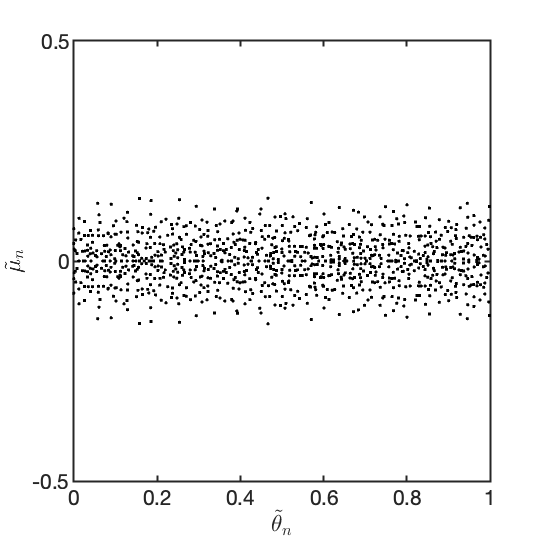
\includegraphics[width=0.45\columnwidth]{spec_k10_gp001_N2001_2x3}}
		{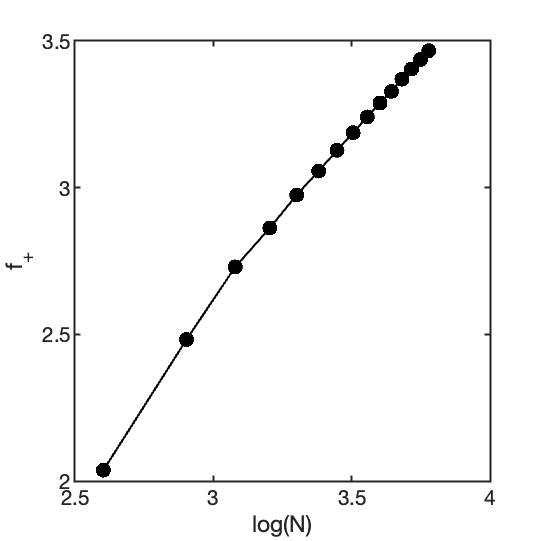
\includegraphics[width=0.45\columnwidth]{fweyl_log_plot_k10_gp001_2x3}}

		\caption{Quasienergy spectrum (left)of the PTKR for K=10}
		\label{fig:ptkr_spec_k10}
	\end{figure}

	
	Equivalently, the total fraction of Planck cells occupied by the gain states, which being mutually orthogonal each occupy a unique Planck cell, will scale in the same way\cite{Henning_2010_frac_weyl}. This is evident in the Husimi distributions of the gain states in the second row of Figure \ref{fig:ptkr_spectrum_husimi_etc_k10}, where we see not only the increased hbar-limited resolution but also the increased localisation due to the fractal scaling of the gain states. In the bottom row of the same figure we show the Husimi dsitribution of the state $\ket{\nu_1}$ , the state with longest lifetime. 
	In the bottom row of Figure \ref{fig:ptkr_spectrum_husimi_etc_k10} we show the classical densities, the classical counterparts of the Husimi distribution. We see an excellent qualitative agreement between the classical densities and their quantum counterparts.
		
	
	
 In the middle row we depict the gain states and see that as we move towards the classical limit the relative fraction of states . This can be seen 
	
	
	

	
	\begin{figure}[h!]
		\centering	
		{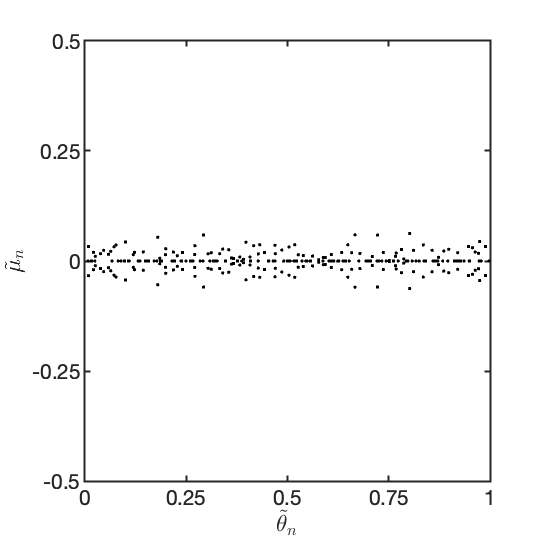
\includegraphics[width=0.24\columnwidth]{spec_k10_gp001_N501_2x3}}
		{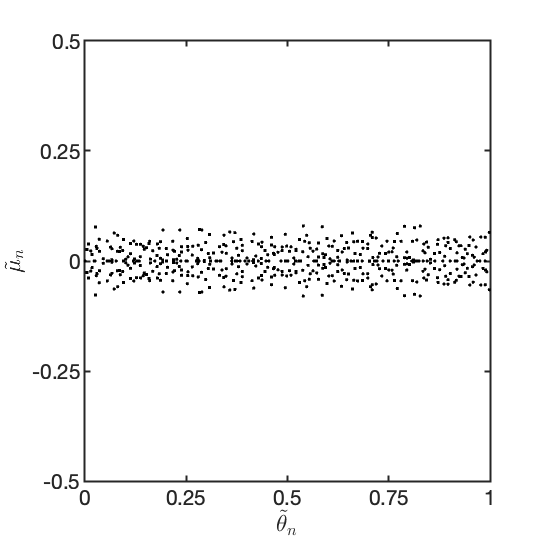
\includegraphics[width=0.24\columnwidth]{spec_k10_gp001_N1001_2x3}}
		{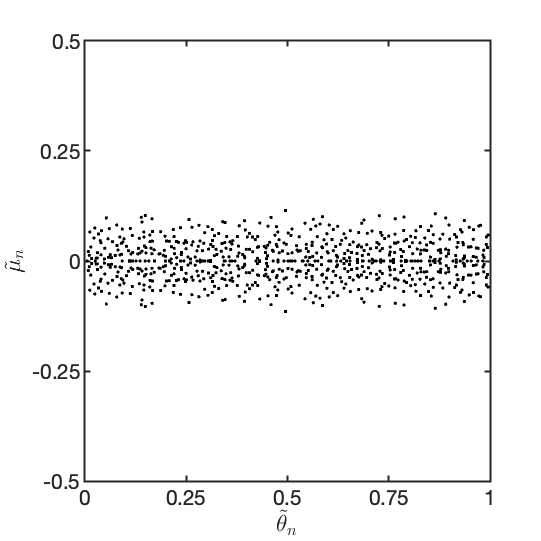
\includegraphics[width=0.24\columnwidth]{spec_k10_gp001_N1501_2x3}}
		{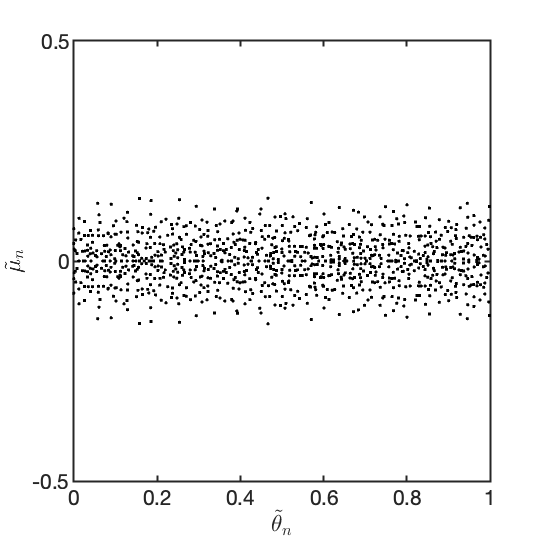
\includegraphics[width=0.24\columnwidth]{spec_k10_gp001_N2001_2x3}}\\
				{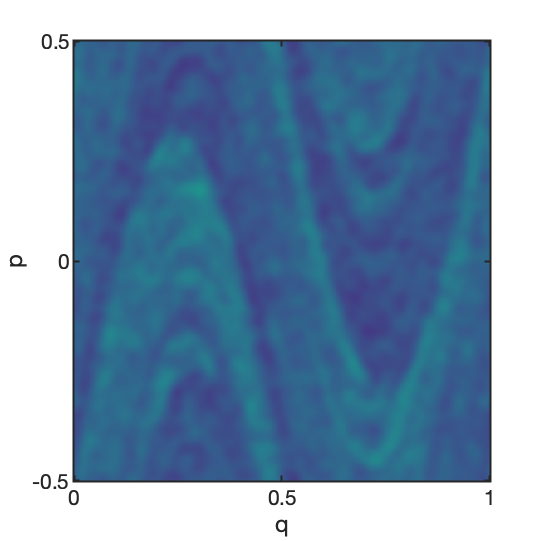
\includegraphics[width=0.24\columnwidth]{ HusG_k10_g0p001_N501_gain_2x3}}
		{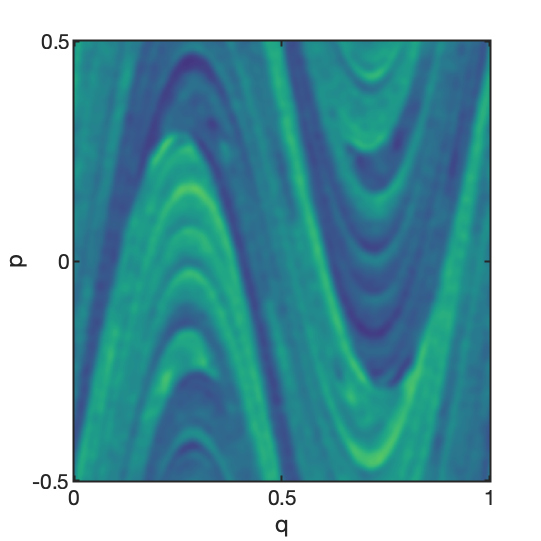
\includegraphics[width=0.24\columnwidth]{ HusG_k10_g0p001_N1001_gain_2x3}}
		{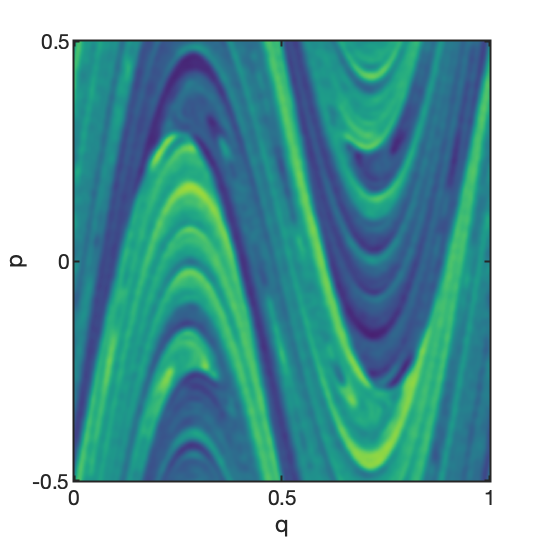
\includegraphics[width=0.24\columnwidth]{ HusG_k10_g0p001_N1501_gain_2x3}}
		{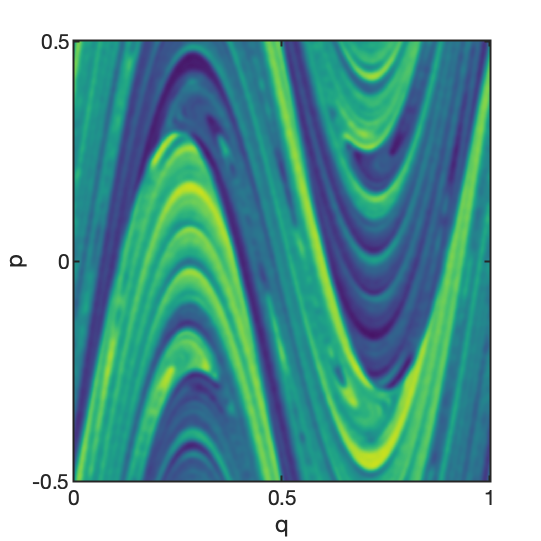
\includegraphics[width=0.24\columnwidth]{ HusG_k10_g0p001_N2001_gain_2x3}}\\
		{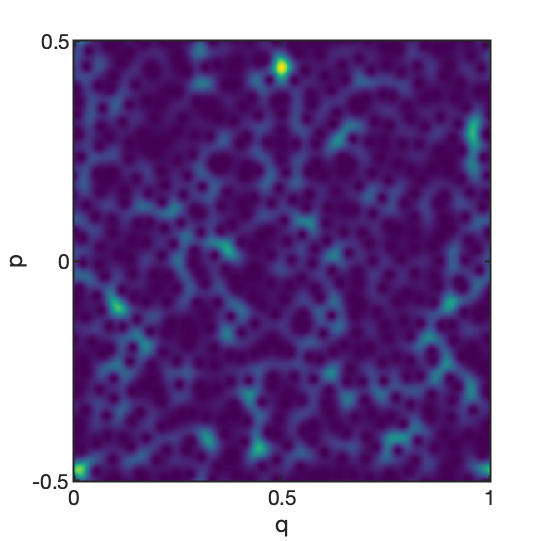
\includegraphics[width=0.24\columnwidth]{ HusG_k10_g0p001_N501_longest_lived_2x3}}
		{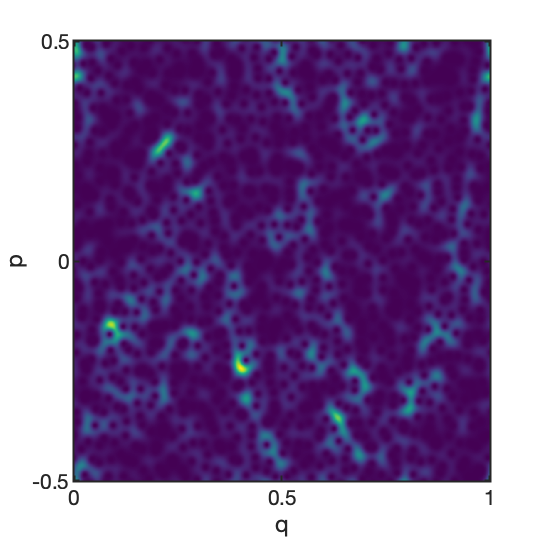
\includegraphics[width=0.24\columnwidth]{ HusG_k10_g0p001_N1001_longest_lived_2x3}}
		{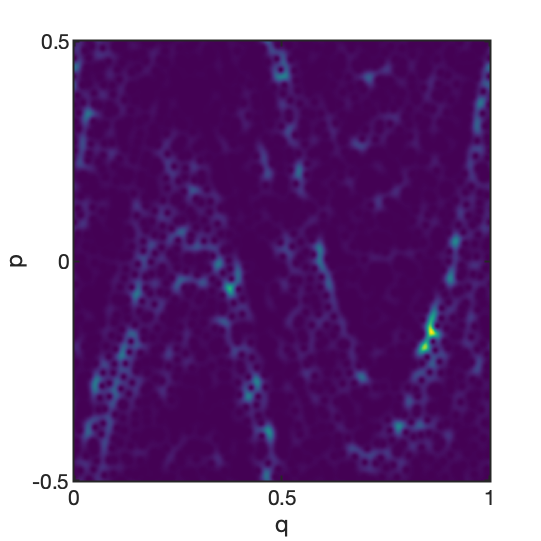
\includegraphics[width=0.24\columnwidth]{ HusG_k10_g0p001_N1501_longest_lived_2x3}}
		{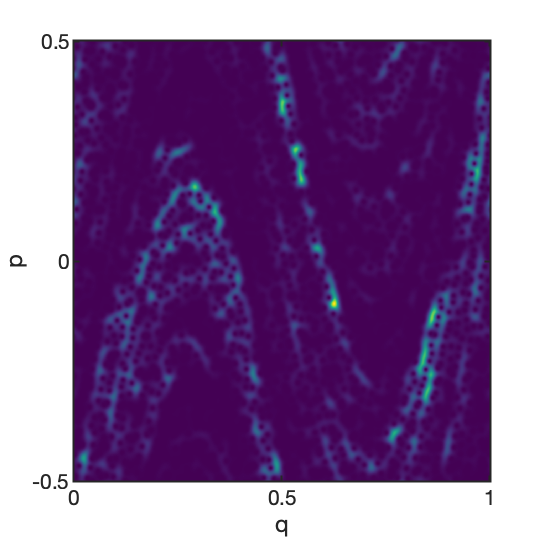
\includegraphics[width=0.24\columnwidth]{ HusG_k10_g0p001_N2001_longest_lived_2x3}}
		\caption{Quasienergy spectrum and Husimi distribution of Schur states for the PT-symmetric kicked rotor with $k=10$, $\gamma=0.001$, and three values of matrix dimension $N=501$ (left), $N=1001$ (middle), and $N=1501$ (right). The top row depicts the quasienergy components rescaled as $\tilde{\mu}=\frac{\mu h}{\gamma}$ and $\tilde{\theta}=\frac{\theta}{\pi}$ . The middle row depicts the Husimi distribution of the Schur state with largest imaginary quasi energy component $\mu_1$. The bottom row depicts the Husimi distribution summed over the set of gain states ($\mu>0$).}
		\label{fig:ptkr_spectrum_husimi_etc_k10}
	\end{figure}
	

	
\begin{figure}[h!]
	\centering	
	{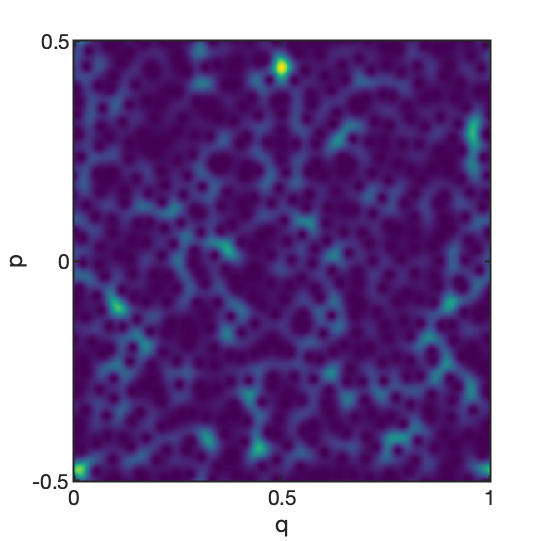
\includegraphics[width=0.24\columnwidth]{ HusG_k10_g0p001_N501_longest_lived_2x3}}
	{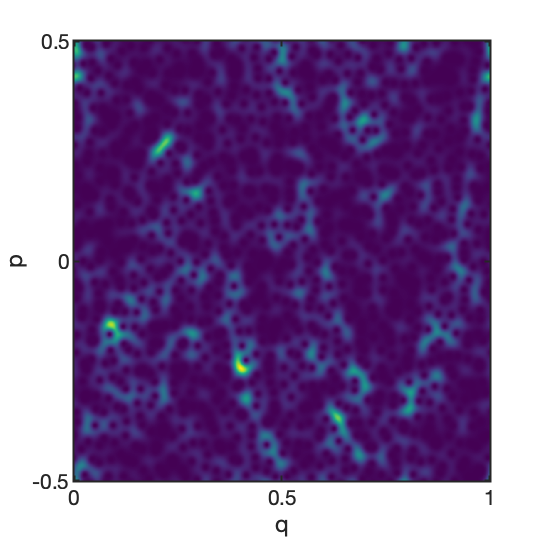
\includegraphics[width=0.24\columnwidth]{ HusG_k10_g0p001_N1001_longest_lived_2x3}}
	{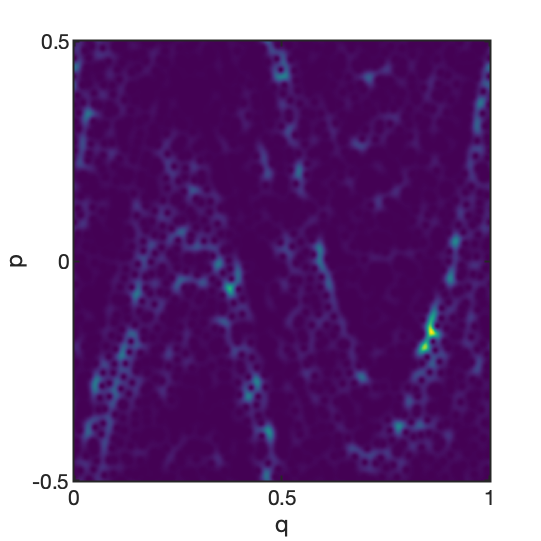
\includegraphics[width=0.24\columnwidth]{ HusG_k10_g0p001_N1501_longest_lived_2x3}}
	{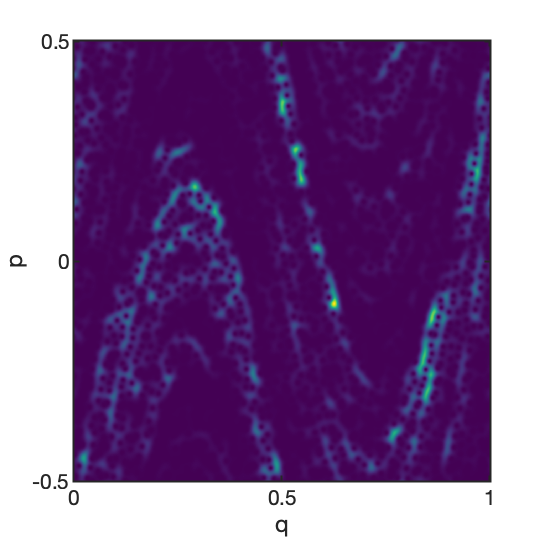
\includegraphics[width=0.24\columnwidth]{ HusG_k10_g0p001_N2001_longest_lived_2x3}}\\
	{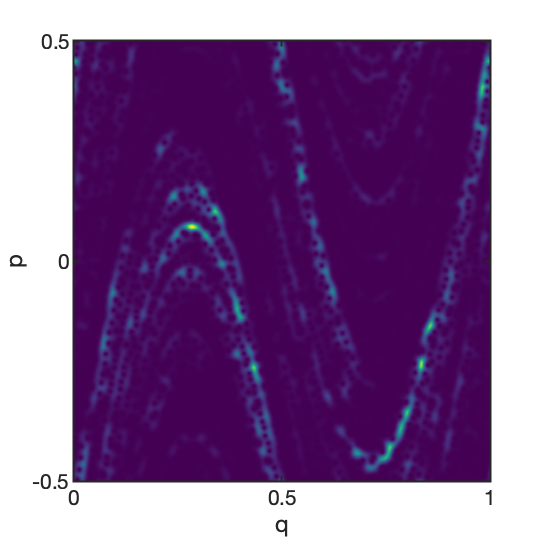
\includegraphics[width=0.24\columnwidth]{ HusG_k10_g0p001_N2501_longest_lived_2x3}}
	{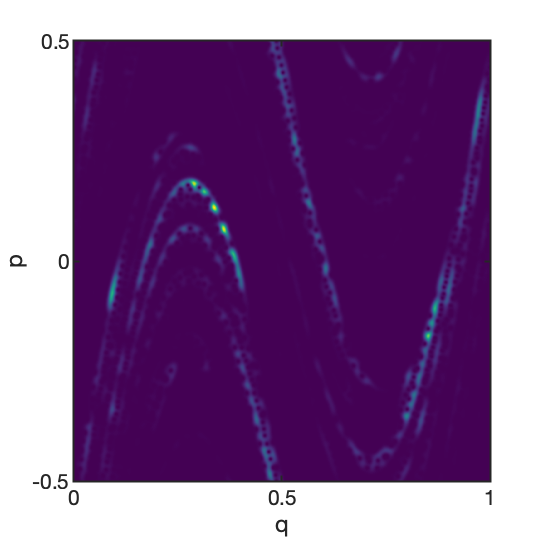
\includegraphics[width=0.24\columnwidth]{ HusG_k10_g0p001_N3501_longest_lived_2x3}}
	{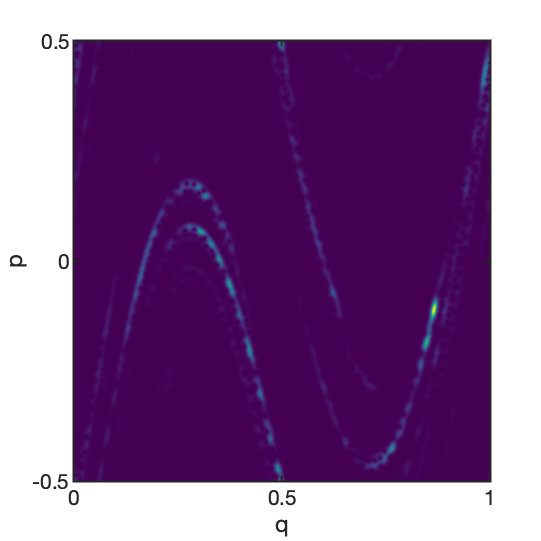
\includegraphics[width=0.24\columnwidth]{ HusG_k10_g0p001_N4001_longest_lived_2x3}}
	{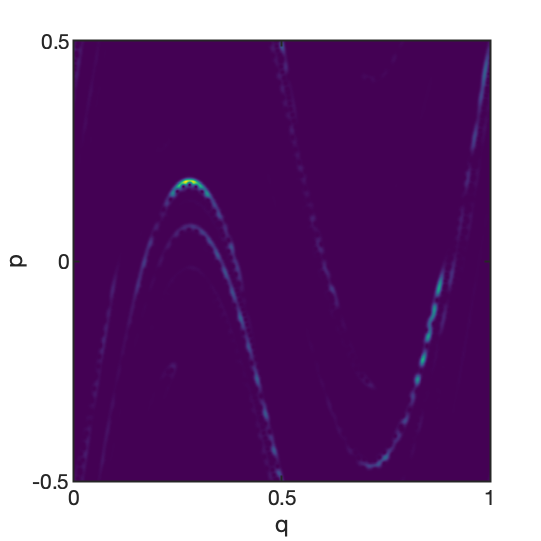
\includegraphics[width=0.24\columnwidth]{ HusG_k10_g0p001_N5001_longest_lived_2x3}}
	
	\caption{Husimi distribution longest lived Schur state $\ket{\nu_1}$ for $k=10$, $\gamma=0.001$ and various $N$. From top left to bottom right $N_1=250$, $500$, $750$,$1000$,$1250$,$1500$,$1750$,$2000$,$2500$}
	\label{fig:ptkr_husimi_k10_longest}
\end{figure}



%
%		We will denote the relative fraction of states belonging to each of these sets as $f_{+}$, $f_{0}$ and $f_{-}$, respectively. We will refer to the fractions $f_{+}$, $f_{0}$, $f_{-}$ as \textit{spectral weights}. We note that because of the PT-symmetry we necessarily have $f_{+}=f_{-}$. In the regime of unbroken PT-symmetry we have $f_0=1$ and $f_{+}=f_{-}=0$. 
%	


\section{Spectral Features and Phase Space}

\begin{itemize}
	\item Size of the spectral gap
	\item could we relate the spectral gap to some kind of classical time for the stable set in rms method?
\end{itemize}

\subsection{Introduction}

One way to view the Weyl law is though the number of Planck cells that are occupied in phase space. For the finite phase space of the kicked rotor their are exactly $N$ Planck cells that can be filled by N orthogonal states.  When the relevant propagator is non-normal, the eigenstates are non-orthogonal and this planck cell partitioning of the phase space fails. However, It was suggested in \cite{Henning_2010_frac_weyl} that a natural way to carry over this idea into the non-normal case was to use the Schur decomposition. The Schur decomposition results in an orthogonal set of eigenfunctions For simple types of open systems with escape through an opening, the Schur decomposition  More recently, we have shown that using 

\subsection{Results}

In terms of the spectral weights $f_{-}$, $f_{0}$, $f_{+}$, introduced in the first section, the standard Weyl law would correspond to each of these being, barring small fluctuations, independent of the matrix dimension. In contrast, in the presence of a fractal Weyl law, we would expect a dependence on the dimension of the Hilbert space $N$, the precise nature of which depends on the proportion of the classical phase space associated to chaotic motion. To investigate this we consider the distribution of the quasienergies $p(\mu)$ defined as 
\begin{equation}
	p(\mu)=\frac{\# (\mu_n>\mu)}{N}
\end{equation}
Here we have rescaled the imaginary parts as $\tilde{\mu}_n=\mu_n\frac{h}{\gamma}$. This rescaling maps the quasienergies into the range $(-0.5,0.5)$. By mapping the quasienergies into this interval we can compare to the exponent of the classical normin the next section. \textcolor{red}{Expand on this}.  

In the top row of Figure \ref{fig:ptkr_pmu_quant} we depict the fraction of quasienergies, $p(\mu)$,  whose imaginary part $\mu_n$  is greater than $\mu$. The various curves depict differing matrix dimension $N=2N_1+1$ where $N_1=250$ (red), $N_1=500$ (blue), $N_1=750$ (green), $N_1=100$ (magenta). We see that when $k=1.1$ the distribution $p(\mu)$ is largely independent of the matrix dimension. In the lower panel, where the distribution over the gain states is show, we observe the majority of the fluctuations happen for small matrix dimension $N=250$. For the higher matrix dimensions the curve charges very little. On the other hand, for the cases $k=5$ (middle) and $k=10$ (right) we observe a rather different behaviour. In each of the cases we see that fraction of stable states, $f_0$, is reduced as the matrix dimension is increased implying an increase in the spectral weight of $f_{+}$. This means that as the matrix dimension is increased the support of the gain set is increasing implying that a fractal scaling is occurring. However this is not the only feature. 
\begin{figure}[h!]
	\centering	
	{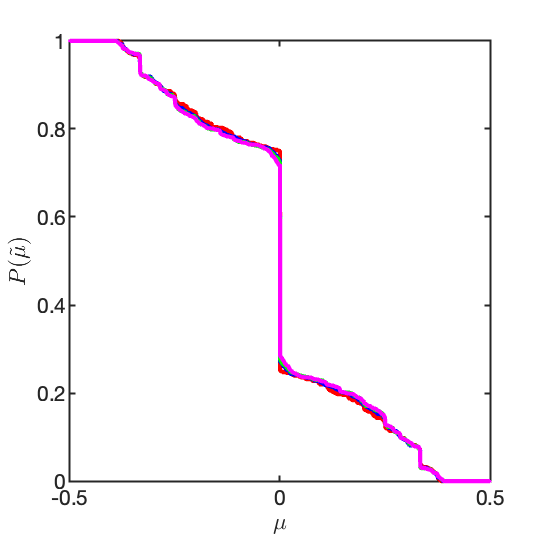
\includegraphics[width=0.32\columnwidth]{pmu_distribution_k1p1_g1_2x3}}
	{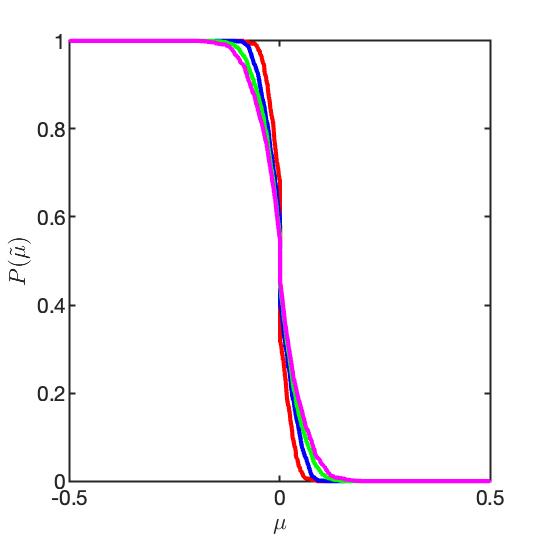
\includegraphics[width=0.32\columnwidth]{pmu_distribution_k5_g1_2x3}}
	{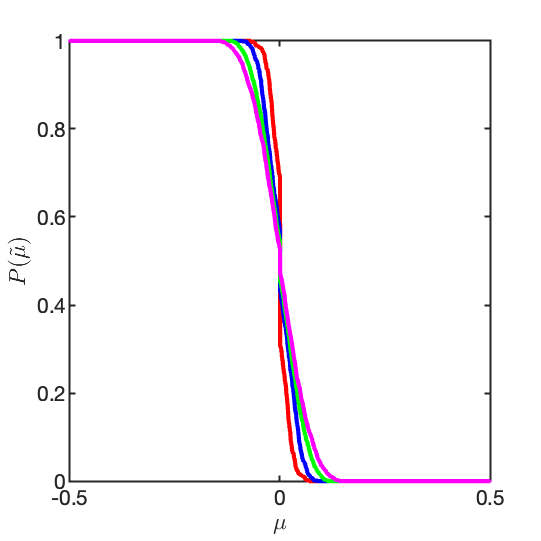
\includegraphics[width=0.32\columnwidth]{pmu_distribution_k10_g1_2x3}}\\
	{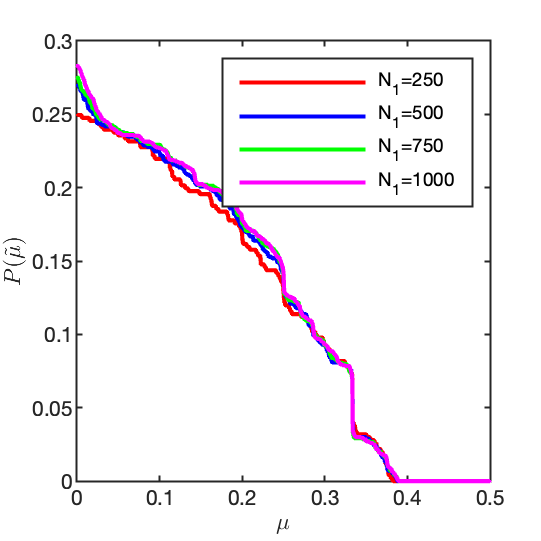
\includegraphics[width=0.32\columnwidth]{pmu_distribution_gain_k1p1_g1_2x3}}
	{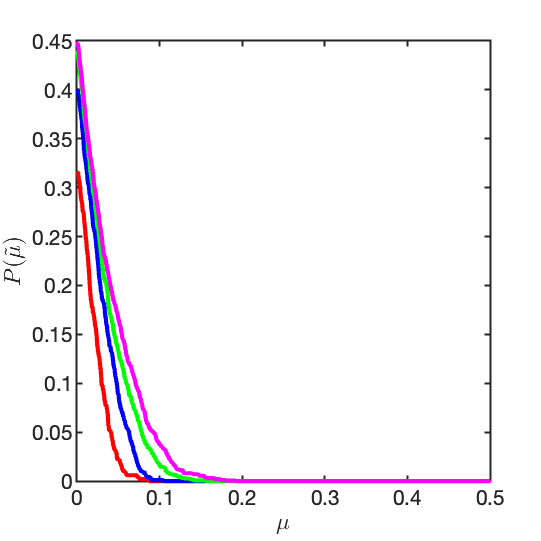
\includegraphics[width=0.32\columnwidth]{pmu_distribution_gain_k5_g1_2x3}}
	{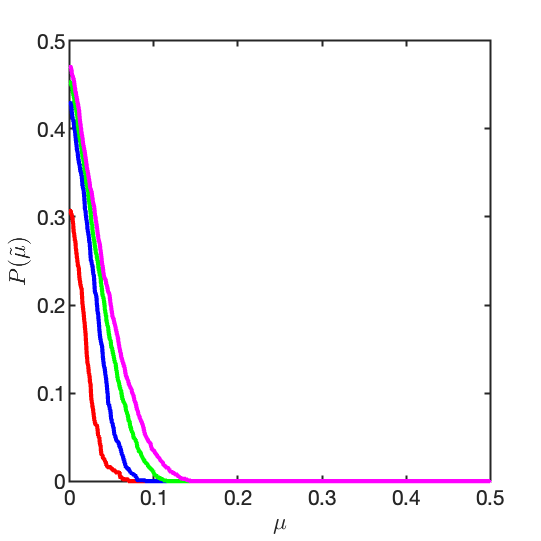
\includegraphics[width=0.32\columnwidth]{pmu_distribution_gain_k10_g1_2x3}}\\
	\caption{Distribution of decay rates $p(\mu)$ in the kicked rotor for  $\gamma=0.001$ for kicking strength $k=1.1$ (left), $k=5$ (middle), and $k=10$ (right) and four values of the matrix dimension  $N=2N_1+1$. The top row depicts the distribution $p(\mu)$ and the bottom row shows just the portion of the distribution where $\mu>0$.}
	\label{fig:ptkr_pmu_quant}
\end{figure}

We also see that the maximum values of the distributions is exploring more of the available $\mu$ range with increasing matrix dimension. To understand the effect of this on the question of what the fractal dimension is lets us consider first how to interpret this scaling of the largest eigenvalue.

\section{The Scaling of the largest eigenvalue}

We see that the distribution of the decay rates is a function of the matrix dimension. In figure \ref{fig:scale_largest_imag} we show the scaling of the largest eigenvalue as a function of the matrix dimension. We see that for the case $k=1.1$ the largest eigenvalue remains largely independent of the matrix dimension. In contrast, for the thee higher kicking strengths we see a non-linear dependence on the largest eigenvalue with the kicking strength. In the right hand plot of the same figure we plot the largest eigenvalue as a function of the kicking strength for three values of the matrix dimension. Again we see that for $k<2$ the largest eigenvalue remains largely independent of the matrix dimension. On the other hand for $k>2$ the largest imaginary part is highly dependent on the matrix dimension. 

\begin{figure}[h!]
	\centering
	{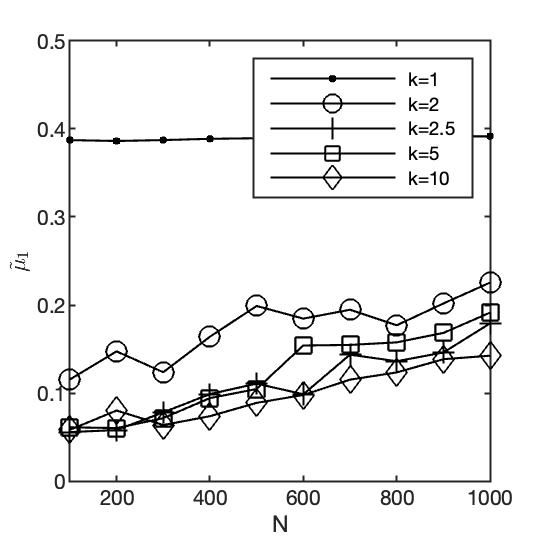
\includegraphics[width=0.45\linewidth]{max_imag_N100_to_N1000_kvals_2x3}}
	{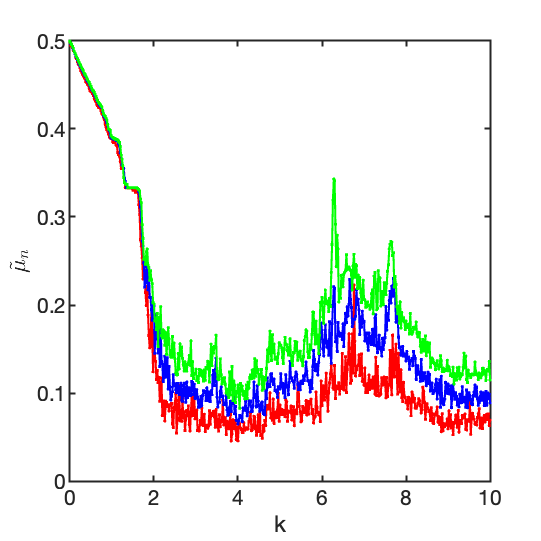
\includegraphics[width=0.45\linewidth]{kick_plot_N500_1000_1500_2x3}}
	\caption{The classical norm parameter $\zeta$ fitted to the quantum data displayed (left) and the corresponding final times (right) for each value of the kicking strength $k$. Red is N=501, Blue N=1001, Green N=1501}
	\label{fig:scale_largest_imag}
\end{figure}

Let us now argue why the trend occurs. In \cite{me} we have shown that a classical counterpart to the Husimi distribution can be constructed via the use of a classical density. We argue that the trend seen in the eigenvalue distribution can be understood based in the maxinmum value of the semi-classical norm. Effectively using the classical density we will extract the largest eigenvalue using a semi-classical expectation value.






\section{Fractal Weyl Law}	

\begin{itemize}
	\item Heat map of the multifractal dimensions $d_q$  overlaying the phase space as a function of $N$
\end{itemize}

For a system with a d-dimensional phase space, the Weyls law approximates the the number of energy states with $\mathcal{N}(E_n<E)\sim E^{\frac{d}{2}}$. Another way to interpret this is that the number of Planck cells that fit in the accessible phase space volume scales as \cite{Henning_2010_frac_weyl,Henning_2013_scattering_PT_Review}. 
\begin{equation}
	\mathcal{N}(h)\propto h^\frac{d}{2}
\end{equation}
where $d\in\mathbb{N}$ is the dimension of the phase space. \textcolor{red}{Mention types of opening and chaotic vs not chaotic}.Opening the system can lead to a modification of the standard Weyl law, giving rise to a non-integer dimension $d\in\mathbb{R^{+}}$, and has been dubbed the fractal weyl law.  The exact nature of dimension and its relation to the underlying classical structures is dependent on the chaos present in the system and the type of opening. 

%In terms of the spectral weights $f_{-}$, $f_{0}$, $f_{+}$, introduced in the first section, the standard Weyl law would correspond to each of these being, barring small fluctuations, independent of the matrix dimension. In contrast, in the presence of a fractal Weyl law we would expect a dependence on the dimension of the Hilbert space $N$, the precise nature of which depends on the chaotic nature of the classical system. We can gain a qualitative estimate of the kicking regimes that will yield a fractal Weyl law by examining these distributions. In the top row of Figure \ref{fig:ptkr_pmu_quant} we depict the fraction of quasienergies, $p(\mu)$,  whose imaginary part $\mu_n$  is greater than $\mu$. The various curves depict differing matrix dimension $N=2N_1+1$ where $N_1=200$ (black), $N_1=400$ (red), $N_1=600$ (green), $N_1=800$ (blue), $N_1=1000$ (magenta). The imaginary parts $\mu_n$ scale with the matrix dimension, to account for this we rescale the eigenvalues in the spectrum by their respective largest imaginary part. This results in imaginary parts falling into the interval $\mu_n\in(-1,1)$.	
%
%
%
%\begin{figure}[h!]
%	\centering	
%	{\includegraphics[width=0.32\columnwidth]{En_distribution_k2_g1_2x3}}
%	{\includegraphics[width=0.32\columnwidth]{En_distribution_k4_g1_2x3}}
%	{\includegraphics[width=0.32\columnwidth]{En_distribution_k10_g1_2x3}}
%	\caption{Distribution of decay rates $p(\mu)$ in the kicked rotor for  $\gamma=0.001$. The matrix dimension is $N=2N_1+1$ with: $N_1=200$ (black), $N_1=400$ (red), $N_1=600$ (green), $N_1=800$ (blue) and $N_1=1000$ (magenta). From left to right and top to bottom: $k=1.1$,$k=5$ and $k=10$.}
%	\label{fig:ptkr_pmu_quant}
%\end{figure}




The dimension of the Husimi distibution of the relevant quantum states can be described through the spectrum of generalised dimensions $\lbrace\mathcal{D}_{q}\rbrace$
\begin{equation}
	\mathcal{D}_{q}=-\lim_{\epsilon\to0} \frac{\log S_\epsilon^{(q)}}{\log \epsilon^{-1}}
\end{equation}
where $\Sfancy^{(q)}$ is the generalised Renyi-entropy
\begin{equation}
	\Sfancy^{(q)}=\frac{1}{1-q}\int \log\left(\mu^q\right)d\mu
\end{equation}
Here the parameter $\epsilon$ is the width of the box that partitions the phase space. In many cases, the present study included, it is common to consider the box-counting dimension $\Dfancy_0$ and the information dimension $\Dfancy_1$. When calculating these for the quantum system the limit x	x

To facilitate a comparison between the quantum and classical values of the $\lbrace \Dfancy_q \rbrace$ it is necessary to restrict the size of the box size to the range $\sqrt{h}<\epsilon<1$. In particular the information dimension $\Dfancy_1$ is trivial for $\epsilon<\sqrt{\hbar}$ and we have $\Dfancy_1(\epsilon<<\sqrt{h})=d$ where $d$ denotes the dimension of the classical phase space.



	
%	\section{The Scaling of the largest eigenvalue}
	
	
%	The main feature of the observed dependence of the largest imaginary part on the kicking strength can be understood by considering the classical norm dynamics. For this purpose we consider the norm map for $k=1.1$, displayed in the right hand plot of Figure \ref{fig:norm_map_forward_reg_mixed}. In the corresponding Poincar\'{e} dynamics we observed that there were islands of regular trajectories confined to the upper and lower momentum plane. Accordingly this confinement means that the classical norm, $w_{n+1}=e^{2\gamma \tilde{p}_{n}}w_n$, will grow/decay monotonically in these regions. For larger values of the kicking strength the classical phase space becomes more chaotic and these regular regions disappear. Thus, trajectories will no longer be confined to these regions of large $|\tilde{p}|$ and the relative rate of maximum norm increase is slower. In Figure \ref{fig:norm_and_imag_vs_kick}, we plot the the rescaled largest imaginary part $\mu_{+}\to\frac{\hbar}{\gamma}\mu_{+}\in(0,0.5]$ for $k\in[0,10]$ in red. \textcolor{red}{lets have a chat about this bit}
%	
%	
%	\begin{figure}
%		\centering
%		{\includegraphics[width=0.4\linewidth]{norm_vs_kick_classical_quant_fit_2x3}}
%		{\includegraphics[width=0.4\linewidth]{norm_vs_kick_final_times_2x3}}
%		\caption{The classical norm parameter $\zeta$ fitted to the quantum data displayed (left) and the corresponding final times (right) for each value of the kicking strength $k$.}
%		\label{fig:norm_and_imag_vs_kick}
%	\end{figure}
%	
%	We argue that the rescaled quantum norm rate $\mu_n=\text{Im}(\epsilon_n)$, reflects this classical norm rate $\zeta:=\ln(w_{n+1})=\frac{\Delta}{\gamma t_f}$ where $\Delta\in\mathbb{R}$ and $t_f={n+1}$.  In Figure \ref{subfig:classical_norm_vs_kick_fitted} we again plot the value of the classical norm but now with different final times for each kicking strength. For each kicking strength the final time, displayed in Figure \ref{subfig:classical_norm_vs_kick_final_times}, is chosen such that it minimises the difference between the quantum $\mu_{+}$ and the classical $\zeta_{+}$
%	
%	


\bibliographystyle{iopart-num}
\bibliography{Ref}	

\appendix



\section{PT Symmetry Breaking}

To investigate the regime of PT-symmetry breaking we consider the spectrum of the Floquet operator $\hat{F}$, with matrix elements \ref{eqn:ptkr_Floquet_matrix_elements}, while varying the classical kicking strength $k$ and the strength $\gamma$ of the gain-loss profile. In terms of the spectral weights introduced above we consider the fraction of quasierngies with non-zero imaginary parts $f_{\pm}=f_{+}+f_{-}$. Clearly the PT-symmetry is in the broken regime whenever $f_{\pm}>0$.  

In Figure \ref{fig:ptkr_brokem_regieme} we show the fraction of quasienergies $f_{\pm}$ with non-zero imaginary parts $\mu_n$ as a function of $k,\gamma$. We consider the kicking interval $k\in[0,10]$ which is significant in the Hermitian limit as it covers the transition from an almost fully regular, to mixed, to chaotic classical dynamics. We will consider four values of $\gamma\in\lbrace10^{-6},10^{-5},10^{-4},10^{-3}\rbrace$ and use a matrix dimension $N=1001$.

The curve $\gamma=10^{-6}$ is initially in the broken phase of PT-symmetry and then returns to the unbroken phase $f_{\pm}=0$ around $k=2$.  The above results seem to indicate that for $\gamma\approx1e-6$ and kicking strength $K>2$ the system is in the regime of unbroken PT-symmetry. In general the regime of unbroken PT-symmetry is independent of the matrix dimension of the problem.\textcolor{red}{Is that true? Examples of yes would by kicked top and SU2 type systems}. In Figure \ref{fig:ptkr_brokem_regieme} we estimate the PT-symmetry breaking parameter $\gamma_c$ as a function of the matrix dimension for various values of the kicking strength. \textcolor{red}{need to do this and add it in}The value of $\gamma_c$ is estimated by a shooting method. We see that  \textcolor{red}{make this figure}

\begin{figure}
	\centering
	{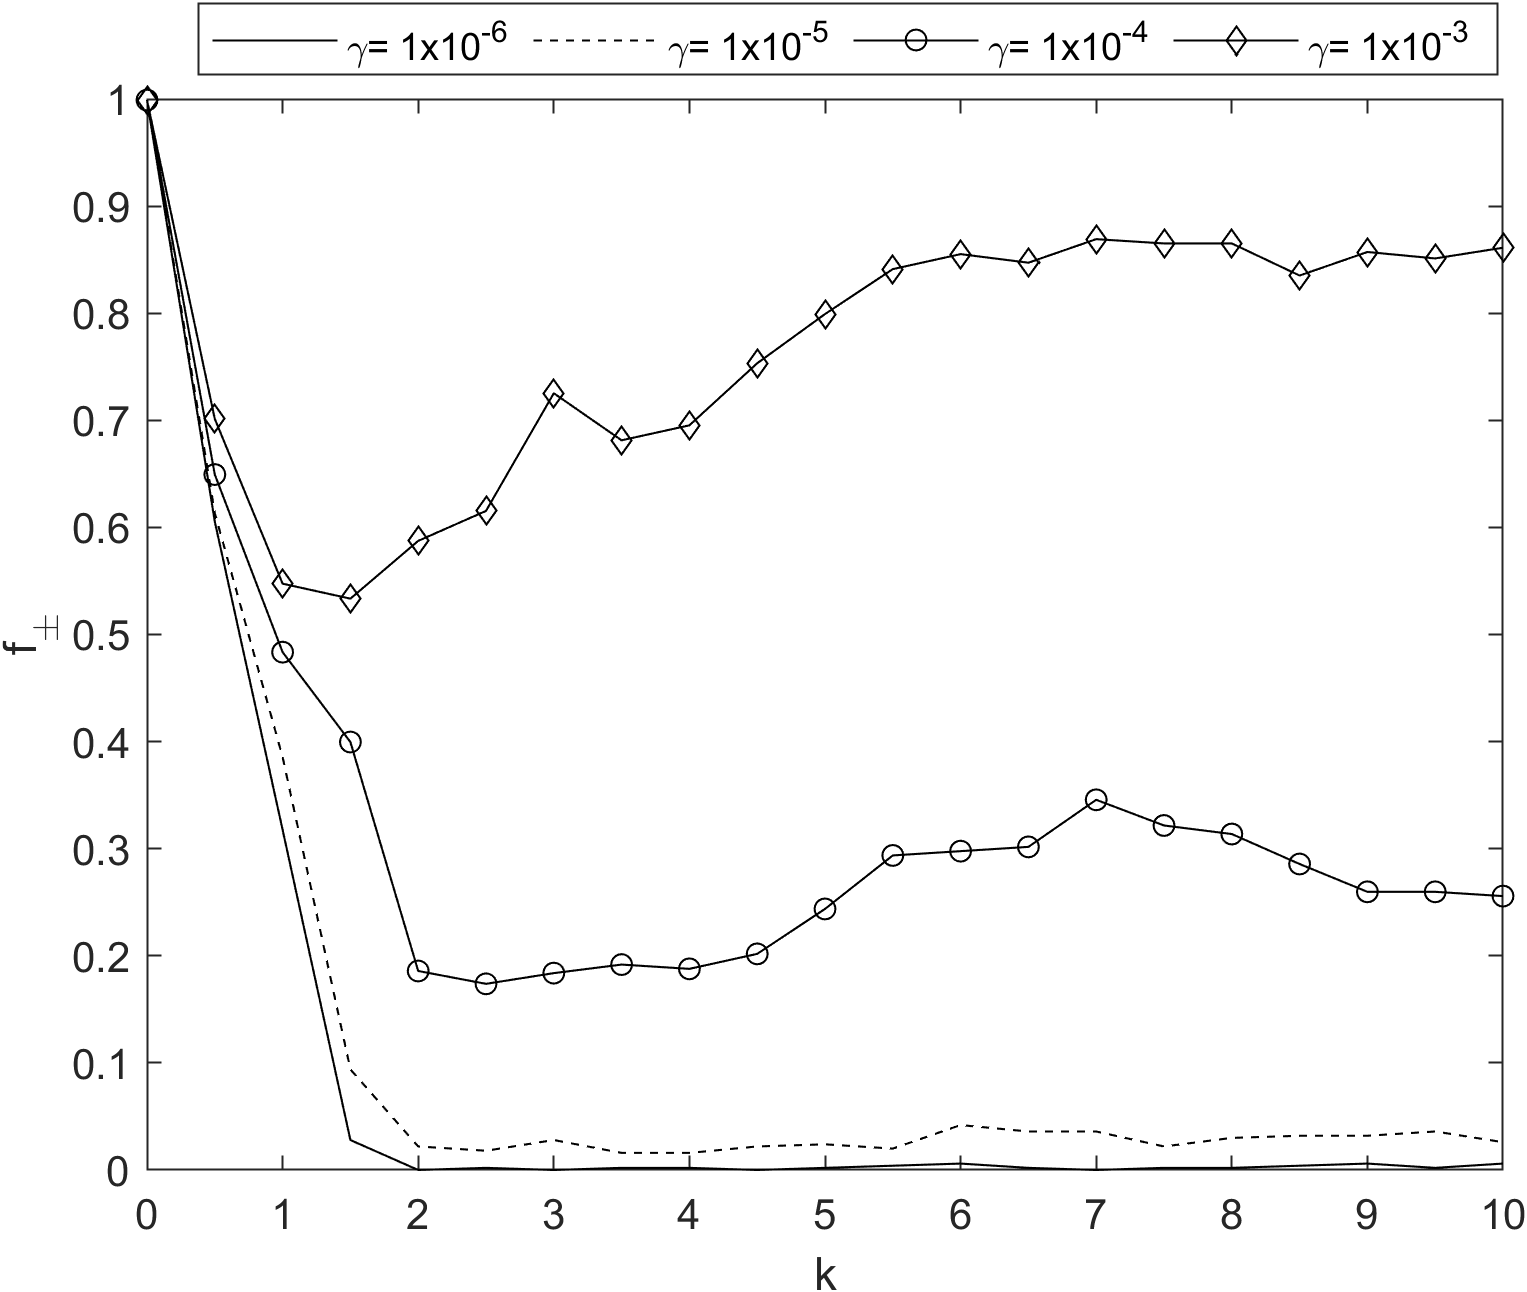
\includegraphics[width=0.5\columnwidth]{PT_Broken_gamma_N500}}
	\caption{Spectral features of the PT-symmetric kicked rotor. The left plot shows the fraction of complex quasienergies in the PT-symmetric kicked rotor as a function of the kicking strength $k$ for various values of $\gamma$. In the right hand plot we show a typical quasienergy spectrum for $k=5$ ad $\gamma=0.001$. In each example the matrix dimension is $N=1001$.}
	\label{fig:ptkr_brokem_regieme}
\end{figure}

For the larger values of $\gamma$ sampled the PT-symmetry is in the broken phase for the entire kicking range. For these values of $\gamma$, we observe that the spectral weight of eigenvalues with real quasienergies $f_0=1-f_{\pm}$ becomes less than the fraction of those with complex quasienergies over the entire kicking range only in the case $\gamma=0.001$.  Let us consider the distributions of the quasienergies in the regime of PT-symmetry breaking. We will focus on the case $\gamma=0.001$ unless otherwise stated but stress that the conclusions apply for other values of $\gamma$.

\section{Constructing the Classical Density}

\end{document}

